\subsection{Метрика Махаланобис}

    Как было показано выше значение критической интенсивности, а знаичт и вероятности выживания попцляции зависит от двух факторов: стохастической чувствительности аттрактора и расстояния до границы бассейна притяжения. Здесь дает ответ следующая метрика. Метрика Махаланобиса показывает расстояние мжду двумя точкасм с учетом стохастической чувствительности аттрактора.

    Метрика Махаланобис рассчитывается по формуле:

    \[d_M = \frac{|x_2^* - x_1^*|}{\sqrt{M}}\]
        
    где \(x_2^*\) --- устойчивое равновесие, либо один из элементов цикла, либо граница хаотического аттрактора. \(x_1^*\) --- либо неустойчивое равновесие, либо его прообраз. \(M\) --- значение функции стохастической чувствительности.

    Графики зависимотстей метрики от параметра \(\beta\) изображены на рисунках \ref{mahalanobis_metrics_alpha_noise}, \ref{mahalanobis_metrics_beta_noise} и \ref{mahalanobis_metrics_additive_noise}

    \comment{Как связаны фсч и критическая интенсивность}

    \comment{Вставь евклидово расстояние}

    \begin{figure}
        \centering
        \subfloat[Для модели (\ref{alpha_chaos})]{
            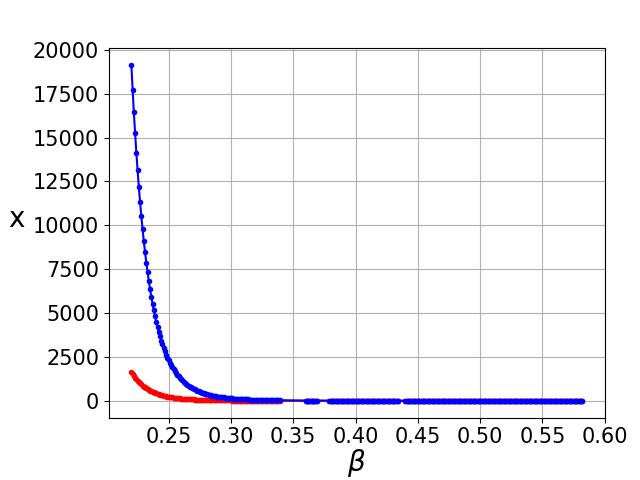
\includegraphics[width=0.55\textwidth]{stochastic/images/mahalanobis_metrics_alpha_noise.jpg}
            \label{mahalanobis_metrics_alpha_noise}
        }
        
        \subfloat[Для модели (\ref{beta_chaos})]{
            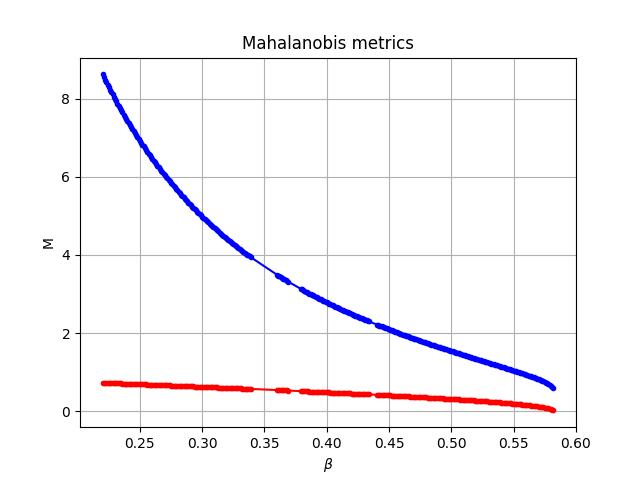
\includegraphics[width=0.55\textwidth]{stochastic/images/mahalanobis_metrics_beta_noise.jpg}
            \label{mahalanobis_metrics_beta_noise}
        }  

        \subfloat[Для модели (\ref{additive_chaos})]{
            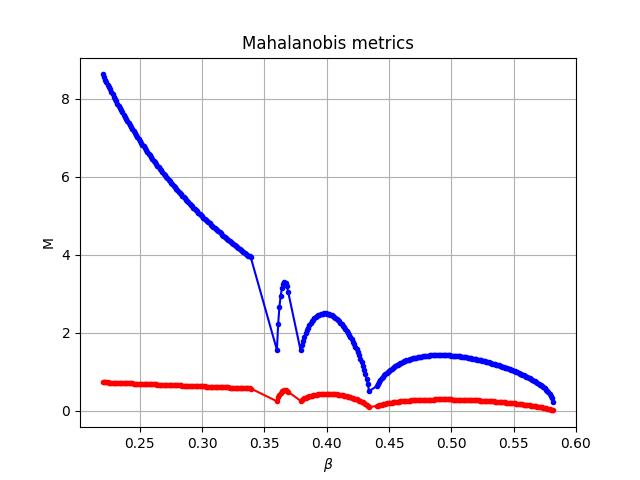
\includegraphics[width=0.55\textwidth]{stochastic/images/mahalanobis_metrics_additive_noise.jpg}
            \label{mahalanobis_metrics_additive_noise}
        }
        
        \caption{Метрика Махаланобис}
    \end{figure}
            